%-----------------------------------------------------------------------------%
\chapter{ANALISIS DAN PERANCANGAN}
%-----------------------------------------------------------------------------%

\vspace{4.5pt}

\section{Analisis Masalah}
\indent
Dalam penelitian ini, sistem kategorisasi akan memiliki data masukan berupa dokumen yang telah diberi label. Dokumen yang akan digunakan adalah dokumen berbentuk penelitian dengan bagian abstrak sebagai fiturnya. Setiap dokumen yang digunakan dapat memiliki lebih dari 1 label ({\itshape multi label}). Label yang diberikan pada setiap dokumen adalah label berupa kategori untuk jenis dokumen penelitian. Label yang digunakan untuk dokumen penelitian adalah {\itshape machine learning}, {\itshape natural language processing}, dan {\itshape image processing}. Data masukan dokumen berabel ini akan digunakan oleh sistem untuk melakukan pengolahan data agar sistem dapat berpikir dan mengambil keputusan seperti layaknya manusia. Jumlah data yang akan digunakan adalah 200 data. Dokumen penelitian akan dibagi menjadi 2 bagian yaitu data {\itshape training} dan data {\itshape testing}. Jumlah data yang digunakan untuk data {\itshape training} adalah 180 data, sedangkan jumlah data untuk data {\itshape testing} adalah 20 data.

\indent
Untuk dapat melakukan hal tersebut, setiap dokumen akan melalui tahap {\itshape pre-processing} terlebih dahulu. Tahap {\itshape pre-processing} ini merupakan tahap untuk memecah sebuah kalimat menjadi sekumpulan kata-kata yang memiliki makna tertentu. {\itshape Pre-processing} akan dimulai dari melakukan {\itshape case folding}, {\itshape filtering}, {\itshape tokenizing}, {\itshape stopword removing}, sampai {\itshape stemming}.

\indent
Setelah menjadi sekumpulan kata-kata, langkah selanjutnya adalah melakukan pemilihan kata yang telah di-{\itshape pre-processing} untuk mengurangi kata-kata yang bobot nilainya rendah. Pemilihan kata-kata ini dapat dilakukan dengan cara pembobotan. Pembobotan ini bertujuan untuk mengurangi jumlah kata yang akan digunakan sistem ketika melakukan pengolahan data agar waktu yang dibutuhkan sistem dapat berkurang. Teknik pembobotan yang akan digunakan dalam penelitian ini adalah TF-IDF.

\indent
Setelah melalui tahap pembobotan, kata-kata yang telah terpilih akan diolah kembali untuk dilakukan pembelajaran ({\itshape learning}) menggunakan salah satu algoritma {\itshape machine learning} yaitu {\itshape Labeled Latent Dirichlet Allocation}. Pembelajaran ini bertujuan untuk menghasilkan suatu model, dimana model ini kemudian akan dijadikan suatu dasar dalam melakukan pengambilan keputusan. Dalam proses pembelajaran menggunakan {\itshape Labeled Latent Dirichlet Allocation} terdapat algoritma tambahan untuk mempermudah rumus perhitungan probabilitas suatu kata. Algoritma tambahan yang digunakan dalam penelitian ini adalah {\itshape Gibbs Sampling}. Model yang dihasilkan oleh algoritma {\itshape Labeled Latent Dirichlet Allocation} adalah berupa matriks probabilitas dokumen terhadap topik ($\theta$) dan matriks probabilitas topik terhadap kata ($\varphi$).

\indent
Setelah proses pembelajaran selesai, model yang telah dihasilkan dapat digunakan untuk proses pengambilan keputusan. Dalam penelitian ini, langkah algoritma yang digunakan untuk pengambilan keputusan adalah {\itshape Simplified Labeled Latent Dirichlet Allocation}. Algoritma ini melakukan pengambilan keputusan hanya dengan menggunakan matriks probabilitas topik terhadap kata saja. Sesuai dengan namanya ({\itshape simplified}), algoritma ini mengambil keputusan tersebut dengan cara melihat kemunculan jumlah kata terbanyak dari dokumen yang diuji dengan kata-kata yang ada di matriks probabilitas topik terhadap kata (20\% kata dengan probabilitas tertinggi pada setiap topik). Jumlah kemunculan kata terbanyak ini bertujuan untuk mengetahui keterkaitan antara kata-kata pada dokumen yang diuji dengan hasil kata-kata pada setiap topik yang telah dilakukan pembelajaran. Setelah mendapatkan kata-kata yang paling berkaitan dengan topik tertentu, maka tetapkan topik tersebut pada dokumen yang sedang diuji. Hasil label dari sistem dapat memiliki lebih dari 1 label ({\itshape multi label}) juga.

\section{Kerangka Pemikiran}
\indent
Gambar 3.1 merupakan gambar yang merepresentasikan kerangka pemikiran dari sistem kategorisasi dokumen yang akan diteliti. Di bawah ini merupakan penjelasan dari kerangka pemikiran pada Gambar 3.1.

\begin{enumerate}[nolistsep,leftmargin=0.5cm]
\item
Proses kategorisasi akan dimulai dengan masukan dataset yang berupa dokumen penelitian, dimana setiap data telah diberikan topik/label terlebih dahulu.
\item
Setelah itu, dokumen penelitian yang telah memiliki label akan dilakukan proses {\itshape pre-processing}. 
\item
Ketika semua data telah melewati proses {\itshape pre-processing}, maka kata-kata yang terdapat pada semua dokumen akan dihitung bobot nilainya dengan TF-IDF. Perhitungan nilai bobot ini berfungsi untuk menyeleksi kata-kata apa saja yang akan digunakan ke dalam proses klasifikasi.
\item
Kata-kata yang terpilih serta label yang telah ditetapkan pada tahap awal kemudian akan diolah untuk dilakukan klasifikasi dengan metode {\itshape Labeled Latent Dirichlet Allocation}.
\item
Pada bagian metode {\itshape Labeled Latent Dirichlet Allocation} terdapat algoritma {\itshape Gibbs Sampling} yang berfungsi untuk melakukan learning dan {\itshape inference} terhadap data yang telah diolah oleh metode {\itshape Labeled Latent Dirichlet Allocation}. Untuk dapat melakukan {\itshape learning} dan {\itshape inference} terdapat beberapa indikator yang perlu ditentukan terlebih dahulu. Indikator ini berupa nilai $\alpha$, $\beta$, jumlah topik, dan jumlah iterasi untuk {\itshape Gibbs Sampling}. Selain itu juga, terdapat beberapa nilai variabel seperti W, Z, $\theta$, dan $\varphi$ yang harus dihitung untuk dapat melakukan {\itshape learning} dan {\itshape inference} menggunakan {\itshape Gibbs Sampling}. 
\item
Hasil dari pengolahan Labeled LDA dan {\itshape Gibbs Sampling} adalah berupa topik/kategori.
\item
Hasil pada bagian 6 dapat diukur dengan menghitung nilai akurasi yang dihasilkan terhadap dokumen penelitian yang diuji. Pengukuran akurasi ini dapat dilakukan dengan menghitung nilai {\itshape precision dan recall}.
\end{enumerate}

\begin{table}[H]
\begin{adjustbox}{width=1\textwidth}
\begin{tabular}{| p {14 cm} |}
\hline
\begin{figure}[H]
	\centering
	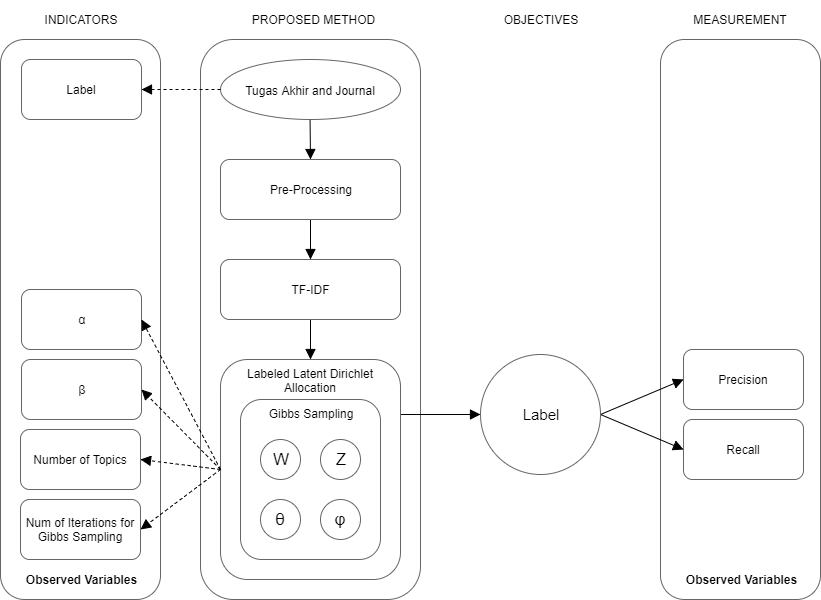
\includegraphics[width=8cm]{images/KerangkaPemikiran}
\end{figure}\\
\hline
\end{tabular}
\end{adjustbox}
\captionof{figure}{Kerangka Pemikiran LLDA}
\end{table}

\section{Perancangan}
\indent
Perancangan merupakan bagian yang menjelaskan urutan proses suatu sistem mulai dari masukan sampai ke keluaran. Pada bagian ini, setiap proses yang telah dijelaskan akan dianalisis secara manual agar lebih mudah untuk memahami setiap proses yang berlangsung selama sistem berjalan. Di bawah ini merupakan {\itshape flowchart} (Gambar 3.2) beserta penjelasan setiap proses untuk sistem klasifikasi dokumen berdasarkan analisis masalah.

\begin{table}[H]
\begin{adjustbox}{width=1\textwidth}
\begin{tabular}{| p {14 cm} |}
\hline
\begin{figure}[H]
	\centering
	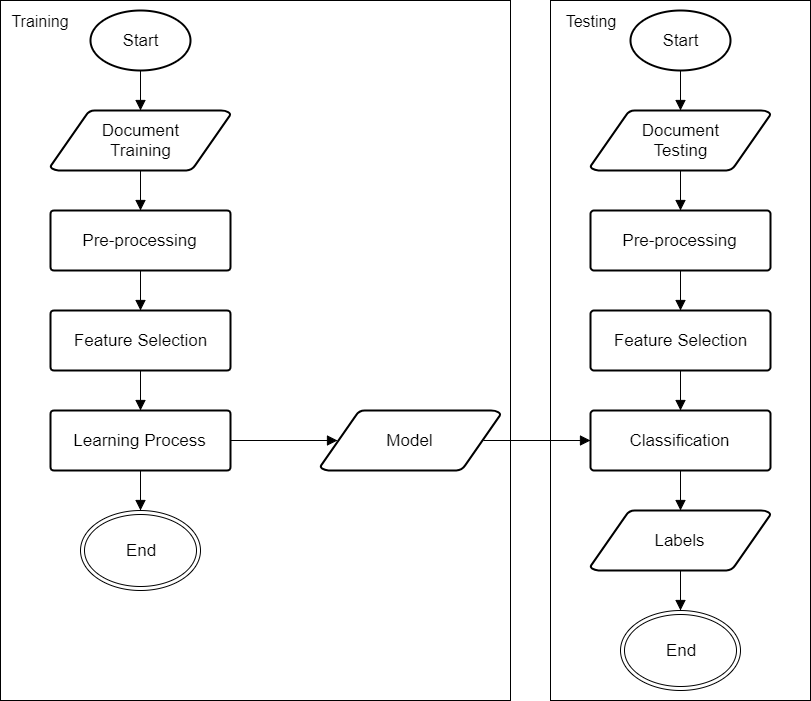
\includegraphics[width=8cm]{images/FlowchartGlobal}
\end{figure}\\
\hline
\end{tabular}
\end{adjustbox}
\captionof{figure}{\textit{Flowchart Global}}
\end{table}

\subsection{{\itshape Data Sampling}}
\indent
Data yang akan digunakan untuk penelitian merupakan data yang bersumber dari IEEE, ACM, {\itshape Research Gate}, dan kampus Institut Teknologi Harapan Bangsa. Data yang didapat kemudian akan direpresentasikan ke dalam {\itshape file} .xls agar lebih mudah dalam pembacaan (terstruktur) dan perubahan data. Di bawah ini merupakan contoh data {\itshape training} maupun {\itshape testing} yang telah direpresentasikan ke dalam {\itshape file} .xls.

\begin{table}[H]
\small
\centering
\caption{Contoh Data dalam {\itshape File} .xls}
\begin{adjustbox}{width=1\textwidth}
\begin{tabular}{| p {1 cm} | p {2 cm} | p {9 cm} | p {2 cm} |}
\hline
{\bfseries Title} & {\bfseries Label} & {\bfseries Content} & {\bfseries Author} \\
\hline
LDA & ML, NLP & Automatically categorizing news articles with high accuracy is an important task in an automated quick news system. & Blei \\
\hline
LLDA & ML, NLP & This paper introduces Labeled LDA, a topic model that constrains Latent Dirichlet Allocation by defining a one-to-one correspondence between LDA’s latent topics and user tags. & Ramage \\
\hline
\end{tabular}
\end{adjustbox}
\end{table}

\noindent
Berikut merupakan karakteristik data abstrak :

\begin{enumerate}[nolistsep,leftmargin=0.5cm]
\item
Menjelaskan masukan, proses, dan keluaran suatu sistem.
\item
Sering muncul kata-kata “menyarankan” atau “menawarkan” ({\itshape proposed}) suatu metode.
\item
Terdapat kalimat mengenai saran pengembangan di kemudian hari.
\end{enumerate}

\begin{table}[H]
\small
\centering
\caption{Jumlah Data {\itshape Training} dan {\itshape Testing}}
\begin{adjustbox}{width=1\textwidth}
\begin{tabular}{| p {8 cm} | p {3 cm} | p {3 cm} |}
\hline
 & {\bfseries Data Training} & {\bfseries Data Testing} \\
\hline
NLP & 40 & 5 \\
\hline
Machine Learning & 25 & 3 \\
\hline
Image Processing & 54 & 5 \\
\hline
NLP dan Machine Learning & 43 & 5 \\
\hline
Machine Learning dan Image Processing & 18 & 2 \\
\hline
\end{tabular}
\end{adjustbox}
\end{table}

\subsection{{\itshape {\itshape Pre-Processing}}}

\begin{table}[H]
\begin{adjustbox}{width=1\textwidth}
\begin{tabular}{| p {14 cm} |}
\hline
\begin{figure}[H]
	\centering
	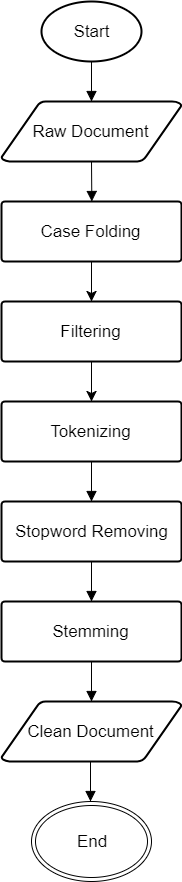
\includegraphics[width=2 cm, height=9 cm]{images/PreProcessing}
\end{figure}\\
\hline
\end{tabular}
\end{adjustbox}
\captionof{figure}{\itshape Flowchart Pre-Processing}
\end{table}

\indent
Pada tahap ini dokumen yang digunakan akan diolah menjadi sekumpulan kata-kata ({\itshape token}) yang kemudian akan digunakan untuk pengolahan data. Keluaran dari tahap {\itshape pre-processing} merupakan daftar kata yang telah diolah menjadi bentuk dasar dan sudah tidak terdapat tanda baca, kata penghubung, kata depan, dll. Untuk melakukan hal tersebut, langkah yang akan dilakukan dalam penelitian ini adalah melakukan {\itshape case folding}, {\itshape filtering}, {\itshape tokenizing}, {\itshape stopword removing}, dan {\itshape stemming}. Gambar 3.3 merupakan alur proses dari tahap {\itshape pre-processing}.


\subsubsection{{\itshape Case Folding}}
\indent
{\itshape Case Folding} digunakan untuk mengurangi jumlah fitur kata yang digunakan. Berdasarkan contoh data pada Tabel 3.1, bagian content dalam data akan dilakukan {\itshape case folding}. Tabel 3.3 merupakan data yang telah melalui tahap {\itshape case folding}.

\begin{table}[H]
\small
\centering
\caption{Hasil {\itshape Case Folding}}
\begin{adjustbox}{width=1\textwidth}
\begin{tabular}{| p {1 cm} | p {2 cm} | p {9 cm} | p {2 cm} |}
\hline
{\bfseries Title} & {\bfseries Label} & {\bfseries Content} & {\bfseries Author} \\
\hline
LDA & ML, NLP & automatically categorizing news articles with high accuracy is an important task in an automated quick news system. & Blei \\
\hline
LLDA & ML, NLP & this paper introduces labeled lda, a topic model that constrains latent dirichlet allocation by defining a one-to-one correspondence between lda’s latent topics and user tags. & Ramage \\
\hline
\end{tabular}
\end{adjustbox}
\end{table}

\subsubsection{{\itshape {\itshape Filtering}}}
\indent
Pada tahap {\itshape filtering}, penghapusan yang dilakukan adalah penghapusan terhadap tanda baca, {\itshape tag}, {\itshape email}, spasi lebih dari 1, dan {\itshape link}. {\itshape Filtering} digunakan untuk mengurangi jumlah fitur kata yang digunakan. {\itshape Filtering} dapat dilakukan dengan menggunakan {\itshape regular expression}. Sebagai contoh berdasarkan Tabel 3.3, bagian {\itshape content} dari setiap dokumen akan dilakukan {\itshape filtering}. Tabel 3.4 merupakan contoh data yang telah melalui tahap {\itshape filtering}.

\begin{table}[H]
\small
\centering
\caption{Hasil {\itshape Filtering}}
\begin{adjustbox}{width=1\textwidth}
\begin{tabular}{| p {1 cm} | p {2 cm} | p {9 cm} | p {2 cm} |}
\hline
{\bfseries Title} & {\bfseries Label} & {\bfseries Content} & {\bfseries Author} \\
\hline
LDA & ML, NLP & automatically categorizing news articles with high accuracy is an important task in an automated quick news system & Blei \\
\hline
LLDA & ML, NLP & this paper introduces labeled lda a topic model that constrains latent dirichlet allocation by defining a one to one correspondence between lda s latent topics and user tags & Ramage \\
\hline
\end{tabular}
\end{adjustbox}
\end{table}

\subsubsection{{\itshape {\itshape Tokenizing}}}
\indent
Pada tahap ini, kata-kata yang telah melalui tahap {\itshape filtering} akan dipecah menjadi kumpulan kata-kata yang disebut sebagai {\itshape token}. Jenis {\itshape tokenizing} yang digunakan pada penelitian ini adalah {\itshape word tokenize}. Sebagai contoh, jika bagian {\itshape content} pada Tabel 3.4 untuk dokumen 1 dilakukan {\itshape tokenizing}, maka hasil yang akan dihasilkan adalah seperti pada Tabel 3.5.

\begin{table}[H]
\small
\centering
\caption{Hasil {\itshape Tokenizing}}
\begin{adjustbox}{width=1\textwidth}
\begin{tabular}{| p {4.666 cm} | p {4.666 cm} | p {4.666 cm} |}
\hline
 \multicolumn{3}{| c |}{\bfseries Kumpulan Kata-kata} \\
\hline
automatically & categorizing & news \\
\hline
articles & with & high \\
\hline
accuracy & is & an \\
\hline
automated & quick & news \\
\hline
system &  &  \\
\hline
\end{tabular}
\end{adjustbox}
\end{table}

\subsubsection{{\itshape {\itshape Stopword Removing}}}
\indent
Pada tahap ini, kata-kata yang telah melalui tahap {\itshape tokenizing} akan dilakukan proses penghapusan terhadap kata-kata yang tidak mewakili makna dari suatu kalimat. {\itshape Stopword removing} bertujuan untuk mengurangi jumlah fitur yang digunakan. Daftar {\itshape stopword} yang digunakan merupakan {\itshape stopword} yang digunakan Google dan bersumber dari www.ranks.nl. Sebagai contoh, Tabel 3.6 merupakan hasil {\itshape stopword removing} terhadap contoh kata-kata pada Tabel 3.5.

\begin{table}[H]
\small
\centering
\caption{Hasil {\itshape Stopword Removing}}
\begin{adjustbox}{width=1\textwidth}
\begin{tabular}{| p {4.666 cm} | p {4.666 cm} | p {4.666 cm} |}
\hline
 \multicolumn{3}{| c |}{\bfseries Kumpulan Kata-kata} \\
\hline
automatically & categorizing & news \\
\hline
articles & accuracy & automated \\
\hline
quick & news & system \\
\hline
\end{tabular}
\end{adjustbox}
\end{table}

\subsubsection{{\itshape {\itshape Stemming}}}
\indent
Pada tahap ini, kata-kata yang telah melalui tahap {\itshape stopword removing} akan diubah menjadi kata dasar sesuai dengan pembentuk katanya. {\itshape Stemming} bertujuan untuk mengurangi jumlah fitur yang digunakan. Proses {\itshape stemming} untuk dokumen berbahasa Inggris akan dilakukan dengan menggunakan algoritma {\itshape Snowball Stemmer}. Tabel 3.7 merupakan contoh hasil {\itshape stemming} terhadap contoh kata-kata pada Tabel 3.6.

\begin{table}[H]
\small
\centering
\caption{Hasil {\itshape Stemming}}
\begin{adjustbox}{width=1\textwidth}
\begin{tabular}{| p {4.666 cm} | p {4.666 cm} | p {4.666 cm} |}
\hline
 \multicolumn{3}{| c |}{\bfseries Kumpulan Kata-kata} \\
\hline
automatic & categorize & news \\
\hline
article & accuracy & automate \\
\hline
quick & news & system \\
\hline
\end{tabular}
\end{adjustbox}
\end{table}

\subsection{{\itshape Feature Selection}}
\indent
Pada tahap ini, kata-kata yang telah di {\itshape pre-processing} akan dihitung bobot nilai dari setiap katanya. Pembobotan ini bertujuan untuk mengurangi jumlah kata yang digunakan selama melakukan pengolahan data. Teknik pembobotan yang akan digunakan dalam penelitian ini adalah TF-IDF. Proses perhitungan TF-IDF yang akan dilakukan di antaranya adalah menghitung nilai TF, DF, dan IDF dengan {\itshape unigram} sebagai jenis {\itshape bag of words}-nya. Gambar 3.4 merupakan alur proses dari penggunaan TF-IDF.

\begin{table}[H]
\begin{adjustbox}{width=1\textwidth}
\begin{tabular}{| p {14 cm} |}
\hline
\begin{figure}[H]
	\centering
	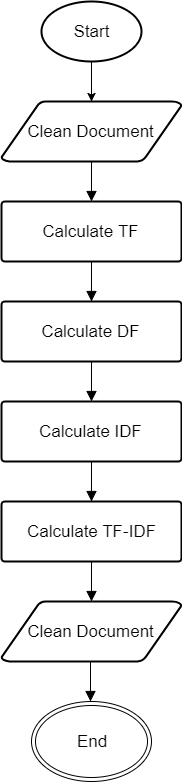
\includegraphics[width=2 cm]{images/FeatureSelection}
\end{figure}\\
\hline
\end{tabular}
\end{adjustbox}
\captionof{figure}{\itshape Flowchart Feature Selection}
\end{table}

\subsubsection{{\itshape Term Frequency}}
\indent
Pada tahap ini, setiap kata dalam suatu dokumen akan dihitung jumlah katanya. Dengan menggunakan Persamaan 2.1, maka kumpulan kata yang telah melalui tahap {\itshape pre-processing} akan digunakan untuk mendapatkan nilai TF. Sebagai contoh pada Tabel 3.8 terdapat 2 dokumen yang telah melalui tahap {\itshape pre-processing}.

\begin{table}[H]
\small
\centering
\caption{Contoh {\itshape Term Count}}
\begin{adjustbox}{width=1\textwidth}
\begin{tabular}{| p {2.8 cm} | p {2.8 cm} | p {2.8 cm} | p {2.8 cm} | p {2.8 cm} |}
\hhline{--~--}
\multicolumn{2}{|c|}{\bfseries Document 1} & \multirow{6}{*}{ } & \multicolumn{2}{|c|}{\bfseries Document 2} \\
\hhline{--~--}
{\bfseries Term} & {\bfseries Term Count} &  & {\bfseries Term} & {\bfseries Term Count} \\
\hhline{--~--}
latent & 3 &  & latent & 2 \\
\hhline{--~--}
topic & 2 &  & topic & 4 \\
\hhline{--~--}
news & 1 &  & credit & 1 \\
\hhline{--~--}
article & 2 &  & tag & 1 \\
\hhline{--~--}
\end{tabular}
\end{adjustbox}
\end{table}

\indent
Tabel 3.8 merupakan tabel yang menunjukan jumlah kata tertentu di suatu dokumen. Langkah selanjutnya adalah melakukan normalisasi terhadap jumlah kata tersebut. Normalisasi ini dilakukan agar nilai bobot yang digunakan ketika perhitungan TF-IDF akan berkisar antara 0 sampai 1. Sebagai contoh, jika kata {\itshape “latent”} pada setiap dokumen akan dihitung nilai TF-nya, maka hasilnya adalah sebagai berikut.

\begin{table}[H]
\small
\centering
\begin{adjustbox}{width=1\textwidth}
\begin{tabular}{| p {14 cm}  |}
\hline
\makecell[l]{
\small{\hspace{40mm}tf("{\itshape latent}", d1) = 3/8 = 0.375}
\\\small{\hspace{40mm}tf("{\itshape latent}", d2) = 2/8 = 0.25}
} \\
\hline
\end{tabular}
\end{adjustbox}
\end{table}

\indent
Sesuai dengan perhitungan di atas untuk kata {\itshape “latent”}, Tabel 3.9 merupakan nilai TF untuk kata-kata yang lain pada dokumen 1 dan 2.

\begin{table}[H]
\small
\centering
\caption{Contoh {\itshape Term Frequency}}
\begin{adjustbox}{width=1\textwidth}
\begin{tabular}{| p {2.8 cm} | p {2.8 cm} | p {2.8 cm} | p {2.8 cm} | p {2.8 cm} |}
\hhline{--~--}
\multicolumn{2}{|c|}{\bfseries Document 1} & \multirow{6}{*}{ } & \multicolumn{2}{|c|}{\bfseries Document 2} \\
\hhline{--~--}
{\bfseries Term} & {\bfseries Term Count} &  & {\bfseries Term} & {\bfseries Term Count} \\
\hhline{--~--}
latent & 0.375 &  & latent & 0.25 \\
\hhline{--~--}
topic & 0.25 &  & topic & 0.5 \\
\hhline{--~--}
news & 0.125 &  & credit & 0.125 \\
\hhline{--~--}
article & 0.25 &  & tag & 0.125 \\
\hhline{--~--}
\end{tabular}
\end{adjustbox}
\end{table}

\subsubsection{{\itshape Document Frequency}}
\indent
{\itshape Document Frequency} (DF) merupakan nilai yang menujukan jumlah dokumen yang memiliki kata tertentu. Untuk menghitung nilai DF, salah satu cara yang dapat dilakukan adalah menggunakan bilangan biner untuk memberikan suatu informasi terhadap semua kata yang terdapat pada setiap dokumen (1 = ada dan 0 = tidak ada).

\begin{table}[H]
\small
\centering
\caption{Contoh Informasi Kata yang Muncul}
\begin{adjustbox}{width=1\textwidth}
\begin{tabular}{| p {4.666 cm} | p {4.666 cm} | p {4.666 cm} |}
\hline
 & {\bfseries Doc 1} & {\bfseries Doc 2} \\
\hline
latent & 1 & 1 \\
\hline
topic & 1 & 1 \\
\hline
news & 1 & 0 \\
\hline
article & 1 & 0 \\
\hline
credit & 0 & 1 \\
\hline
tag & 0 & 1 \\
\hline
\end{tabular}
\end{adjustbox}
\end{table}

\indent
Setelah memberikan informasi dengan bilangan biner untuk setiap kata pada semua dokumen, langkah selanjutnya adalah menjumlahkan semua bilangan biner pada semua dokumen untuk setiap kata.

\begin{table}[H]
\small
\centering
\caption{Contoh {\itshape Document Frequency}}
\begin{adjustbox}{width=1\textwidth}
\begin{tabular}{| p {3.5 cm} | p {3.5 cm} | p {3.5 cm} | p {3.5 cm} |}
\hline
{\bfseries Term} & {\bfseries Doc 1} & {\bfseries Doc 2} & {\bfseries DF} \\
\hline
latent & 1 & 1 & 2 \\
\hline
topic & 1 & 1 & 2 \\
\hline
news & 1 & 0 & 1 \\
\hline
article & 1 & 0 & 1 \\
\hline
credit & 0 & 1 & 1 \\
\hline
tag & 0 & 1 & 1 \\
\hline
\end{tabular}
\end{adjustbox}
\end{table}

\subsubsection{{\itshape Inverse Document Frequency}}
\indent
{\itshape Inverse Document Frequency} (IDF) merupakan nilai yang digunakan untuk meningkatkan bobot nilai suatu kata yang tidak terlalu sering muncul dan mengurangi bobot yang sering muncul. Dengan menggunakan Persamaan 2.2, maka nilai IDF pada contoh tabel 3.12 adalah sebagai berikut.

\begin{table}[H]
\small
\centering
\caption{Contoh {\itshape Inverse Document Frequency}}
\begin{adjustbox}{width=1\textwidth}
\begin{tabular}{| p {4 cm} | p {4 cm} | p {6 cm} |}
\hline
{\bfseries Term} & {\bfseries DF} & {\bfseries IDF} \\
\hline
latent & 2 & log(2/2) = 0 \\
\hline
topic & 2 & log(2/2) = 0  \\
\hline
news & 1 & log(2/1) = 0.301 \\
\hline
article & 1 & log(2/1) = 0.301 \\
\hline
credit & 1 & log(2/1) = 0.301 \\
\hline
tag & 1 & log(2/1) = 0.301  \\
\hline
\end{tabular}
\end{adjustbox}
\end{table}

\subsubsection{TF-IDF}
\indent
TF-IDF merupakan nilai yang menunjukan seberapa informatif suatu kata muncul di setiap dokumen. Semakin tinggi nilai TF-IDF pada suatu kata, maka semakin informatif juga kata tersebut pada suatu dokumen. Jika kata {\itshape “latent”} pada setiap dokumen akan dihitung nilai TF-IDF-nya, maka hasilnya adalah sebagai berikut.

\begin{table}[H]
\small
\centering
\begin{adjustbox}{width=1\textwidth}
\begin{tabular}{| p {14 cm}  |}
\hline
\makecell[l]{
\small{\hspace{40mm}tfidf("{\itshape latent}", d1) = 0.375 * 0 = 0}
\\\small{\hspace{40mm}tfidf("{\itshape latent}", d2) = 0.25 * 0 = 0}
} \\
\hline
\end{tabular}
\end{adjustbox}
\end{table}

\indent
Sesuai dengan perhitungan di atas untuk kata {\itshape “latent”}, Tabel 3.13 merupakan nilai TF-IDF untuk kata-kata yang lain pada dokumen 1 dan 2 pada Tabel 3.8.

\begin{table}[H]
\small
\centering
\caption{Contoh TF-IDF}
\begin{adjustbox}{width=1\textwidth}
\begin{tabular}{| p {2.333 cm} | p {2.333 cm} | p {2.333 cm} | p {2.333 cm} | p {2.333 cm} | p {2.333 cm} |}
\hline
\multirow{2}{*}{{\bfseries Term}} & \multicolumn{2}{|c|}{{\bfseries TF}} & \multirow{2}{*}{{\bfseries IDF}} & \multicolumn{2}{|c|}{{\bfseries TF-IDF}} \\
\hhline{~--~--}
 & {\bfseries Doc} 1 & {\bfseries Doc 2} &  & {\bfseries Doc 1} & {\bfseries Doc 2} \\
\hline
latent & 0.375 & 0.25 & 0 & 0 & 0 \\
\hline
topic & 0.25 & 0.5 & 0 & 0 & 0 \\
\hline
news & 0.125 & 0 & 0.301 & 0.037625 & 0 \\
\hline
article & 0.25 & 0 & 0.301 & 0.07525 & 0 \\
\hline
credit & 0 & 0.125 & 0.301 & 0 & 0.037625 \\
\hline
tag & 0 & 0.125 & 0.301 & 0 & 0.037625 \\
\hline
\end{tabular}
\end{adjustbox}
\end{table}

\indent
Setelah mendapatkan nilai TF-IDF, langkah selanjutnya adalah melakukan pemilihan kata berdasarkan nilai TF-IDF tersebut. Pemilihan kata ini dilakukan dengan cara mengambil n TF-IDF tertinggi. Sebagai contoh, kata akan dipilih dengan mengambil 2 TF-IDF tertinggi. Berdasarkan nilai TF-IDF pada Tabel 3.13, 2 TF-IDF tertinggi terletak pada kata {\itshape “news”}, {\itshape “article”}, {\itshape “credit”}, dan “{\itshape tag}”. Nilai TF-IDF untuk kata {\itshape “news”}, {\itshape “credit”}, dan “{\itshape tag}” adalah bernilai sama, sehingga kata yang akan dipilih adalah kata yang terlebih dahulu dilakukan pengecekan (dilakukan dari dokumen 1 dan untuk kata-kata dicek dari yang paling atas ke bawah). Oleh karena itu, kata yang akan dipilih berdasarkan 2 TF-IDF tertinggi adalah kata {\itshape “news”} dan {\itshape “article”}. Setelah mendapatkan kata-kata yang terpilih, langkah selanjutnya adalah melakukan pemeriksaan setiap kata pada semua dokumen dengan kondisi jika terdapat suatu kata yang tidak terpilih dari 2 TF-IDF tertinggi, maka kata tersebut akan dihapus (selain kata {\itshape “news”} dan {\itshape “article”}).

\subsection{{\itshape Learning Process}}
\indent
{\itshape Learning Process} merupakan bagian yang menjelaskan langkah serta perhitungan dari penggunaan algoritma untuk menghasilkan {\itshape classifier model}. Algoritma yang akan digunakan pada penelitian ini adalah {\itshape Simplified Labeled Latent Dirichlet Allocation Classifier} (SLLDA-C). Langkah-langkah untuk menggunakan SLLDA-C dapat dilihat pada bab 2 bagian 2.1.10. Berdasarkan langkah SLLDA-C pada bagian 3.3.4 ini, langkah yang akan dijelaskan hanya pada sampai langkah ke-2 saja, karena langkah ke-1 sampai langkah ke-2 merupakan langkah untuk menghasilkan {\itshape classifier model} sedangkan langkah ke-3 dan ke-4 merupakan langkah untuk pengujian. Berikut merupakan contoh penggunaan SLLDA-C.

\begin{enumerate}[nolistsep,leftmargin=0.5cm]
\item
Siapkan dokumen yang akan dijadikan sebagai data {\itshape training}, dimana setiap dokumen telah diberi label terlebih dahulu. Lalu simpan label beserta isi dokumen ke dalam sebuah {\itshape file} (.xls).

\begin{table}[H]
\small
\centering
\caption{Contoh Isi Dokumen Beserta Label}
\begin{adjustbox}{width=1\textwidth}
\begin{tabular}{| p {2 cm} | p {7 cm} | p {5 cm} |}
\hline
 & \textbf{Kata-kata} & \textbf{Label} \\
\hline
Doc 1 & classify, recommend, classify & NLP, ML \\
\hline
Doc 2 & image, classify & ML, Citra \\
\hline
Doc 3 & text, text & NLP \\
\hline
\end{tabular}
\end{adjustbox}
\end{table}

\item
Tetapkan nilai $\alpha$, $\beta$, jumlah label (K), dan jumlah iterasi untuk digunakan ketika proses pembelajaran berlangsung. Nilai $\alpha$ dan $\beta$ memiliki nilai {\itshape default} yaitu 50/K dan 0.1 [10].

\begin{table}[H]
\small
\centering
\caption{Contoh Nilai Masukan LLDA}
\begin{adjustbox}{width=1\textwidth}
\begin{tabular}{| p {4 cm} | p {4 cm} | p {6 cm} |}
\hline
 & \textbf{Default} & \textbf{Nilai yang akan digunakan} \\
\hline
K & - & 3 $\rightarrow$ [NLP, ML, Citra] \\
\hline
$\alpha$ & 50/K & 16.67\\
\hline
$\beta$ & 0.1 & 0.1 \\
\hline
Jumlah Iterasi & 1000 & 1000 \\
\hline
\end{tabular}
\end{adjustbox}
\end{table}

\item
Mencari nilai $\Lambda$ dengan melihat label pada setiap dokumen. Langkah ini merupakan langkah pada {\itshape Pseudocode} 2.2 baris 5. Nilai $\Lambda$ merupakan nilai yang menujukkan ada tidaknya topik tersebut pada setiap dokumen. Bilangan yang digunakan merupakan bilangan biner, dimana angka 1 menunjukan bahwa suatu dokumen memiliki topik tersebut dan angka 0 menunjukan suatu dokumen tidak memiliki topik tersebut.

\begin{table}[H]
\small
\centering
\caption{Contoh Pemetaan Ada Tidaknya Suatu Topik Pada Setiap Dokumen}
\begin{adjustbox}{width=1\textwidth}
\begin{tabular}{| p {3 cm} | p {11 cm} |}
\hline
\textbf{$\Lambda^{(d)}$} & \textbf{Nilai $\rightarrow$ $\lbrace$ NLP, ML, Citra $\rbrace$} \\
\hline
$\Lambda^{(1)}$ & $\lbrace$ 1, 1, 0 $\rbrace$ \\
\hline
$\Lambda^{(2)}$ & $\lbrace$ 0, 1, 1 $\rbrace$  \\
\hline
$\Lambda^{(3)}$ & $\lbrace$ 1, 0, 0 $\rbrace$  \\
\hline
\end{tabular}
\end{adjustbox}
\end{table}

\item
Lakukan pengindeksan untuk setiap kata yang unik yang terdapat pada setiap dokumen. Kata yang sama memiliki indeks yang sama.

\begin{table}[H]
\small
\centering
\caption{Contoh Hasil Pengindeksan Terhadap Semua Kata}
\begin{adjustbox}{width=1\textwidth}
\begin{tabular}{| p {3 cm} | p {6 cm} | p {5 cm} |}
\hline
 & \textbf{Kata-kata} & \textbf{Indeks Kata} \\
\hline
\multirow{3}{*}{\bfseries Doc 1} & classify & 1 \\
\hhline{~--}
 & recommend & 2 \\
\hhline{~--}
 & classify & 1 \\
\hline
\multirow{2}{*}{\bfseries Doc 2} & image & 3 \\
\hhline{~--}
& classify & 1 \\
\hline
\multirow{2}{*}{\bfseries Doc 3}& text & 4 \\
\hhline{~--}
& text & 4 \\
\hline
\end{tabular}
\end{adjustbox}
\end{table}

\item
Siapkan matriks untuk menampung jumlah topik terhadap kata ({\itshape topic-word}), dokumen terhadap topik ({\itshape document-topic}), dan {\itshape topic assignment} ({\itshape document-word}).

\begin{table}[H]
\small
\centering
\caption{Contoh Matriks Awal Jumlah Topik Terhadap Kata}
\begin{adjustbox}{width=1\textwidth}
\begin{tabular}{| p {2.8 cm} | p {2.8 cm} | p {2.8 cm} | p {2.8 cm} | p {2.8 cm} |}
\hline
 \multicolumn{5}{|c|}{\bfseries Topic-Word} \\
\hline
 & {\bfseries classify} & {\bfseries recommend} & {\bfseries image} & {\bfseries text} \\
\hline
{\bfseries NLP} & 0 & 0 & 0 & 0 \\
\hline
{\bfseries ML} & 0 & 0 & 0 & 0 \\
\hline
{\bfseries Citra} & 0 & 0 & 0 & 0 \\
\hline
\end{tabular}
\end{adjustbox}
\end{table}

\begin{table}[H]
\small
\centering
\caption{Contoh Matriks Awal Jumlah Dokumen Terhadap Topik}
\begin{adjustbox}{width=1\textwidth}
\begin{tabular}{| p {3.5 cm} | p {3.5 cm} | p {3.5 cm} | p {3.5 cm} |}
\hline
 \multicolumn{4}{|c|}{\bfseries Document-Topic} \\
\hline
 & {\bfseries ML} & {\bfseries NLP} & {\bfseries Citra} \\
\hline
{\bfseries Doc 1} & 0 & 0 & 0 \\
\hline
{\bfseries Doc 2} & 0 & 0 & 0 \\
\hline
{\bfseries Doc 3} & 0 & 0 & 1 \\
\hline
\end{tabular}
\end{adjustbox}
\end{table}

\begin{table}[H]
\small
\centering
\caption{Contoh Awal Penetapan Topik Terhadap Semua Kata}
\begin{adjustbox}{width=1\textwidth}
\begin{tabular}{| p {3 cm} | p {6 cm} | p {5 cm} |}
\hline
 \multicolumn{3}{|c|}{\bfseries Topic Assignment} \\
\hline
 & Kata-kata & Indeks Topik \\
\hline
\multirow{3}{*}{\bfseries Doc 1} & classify & 0 \\
\hhline{~--}
 & recommend & 0 \\
\hhline{~--}
 & classify & 0 \\
\hline
\multirow{2}{*}{\bfseries Doc 2} & image & 0 \\
\hhline{~--}
 & classify & 0 \\
\hline
\multirow{2}{*}{\bfseries Doc 3}& text & 0 \\
\hhline{~--}
 & text & 0 \\
\hline
\end{tabular}
\end{adjustbox}
\end{table}

\item
Menetapkan topik secara acak untuk setiap kata yang terdapat pada setiap dokumen. Ketika setiap kata diberikan sebuah topik, tambahkan ({\itshape increment}) jumlah kata dengan topik tersebut pada kolom dan baris yang sesuai pada matriks {\itshape topic-word}. Selain itu juga, lakukan perubahan nilai pada matriks {\itshape topic assignment} dengan melihat dokumen serta kata yang sesuai dengan indeks topik yang didapat. Langkah ini dilakukan untuk mengganti nilai $\theta$ yang belum pernah dihasilkan sebelumnya ({\itshape Pseudocode} 2.2 pada baris 7).

\begin{table}[H]
\small
\centering
\caption{Contoh Hasil Random Topic Untuk Semua Kata}
\begin{adjustbox}{width=1\textwidth}
\begin{tabular}{| p {3 cm} | p {6 cm} | p {5 cm} |}
\hline
 \multicolumn{3}{|c|}{\bfseries Topic Assignment} \\
\hline
 & Kata-kata & Indeks Topik \\
\hline
\multirow{3}{*}{\bfseries Doc 1} & classify & 2 \\
\hhline{~--}
 & recommend & 2 \\
\hhline{~--}
 & classify & 1 \\
\hline
\multirow{2}{*}{\bfseries Doc 2} & image & 3 \\
\hhline{~--}
& classify & 2 \\
\hline
\multirow{2}{*}{\bfseries Doc 3}& text & 2 \\
\hhline{~--}
& text & 1 \\
\hline
\end{tabular}
\end{adjustbox}
\end{table}


\begin{table}[H]
\small
\centering
\caption{Contoh Hasil Penambahan Nilai Matriks {\itshape Topic-Word}}
\begin{adjustbox}{width=1\textwidth}
\begin{tabular}{| p {2.8 cm} | p {2.8 cm} | p {2.8 cm} | p {2.8 cm} | p {2.8 cm} |}
\hline
 \multicolumn{5}{|c|}{\bfseries Topic-Word} \\
\hline
 & {\bfseries classify} & {\bfseries recommend} & {\bfseries image} & {\bfseries text} \\
\hline
{\bfseries NLP} & 1 & 0 & 0 & 1 \\
\hline
{\bfseries ML} & 2 & 1 & 0 & 1 \\
\hline
{\bfseries Citra} & 0 & 0 & 1 & 0 \\
\hline
\end{tabular}
\end{adjustbox}
\end{table}

\item
Setelah matriks {\itshape topic assignment} dan {\itshape topic-word} terisi, langkah selanjutnya adalah mengisi matriks {\itshape document-topic}. Nilai dari matriks {\itshape document-topic} merupakan jumlah kata pada suatu topik yang terdapat pada setiap dokumen. Untuk mempermudah perhitungan nilai pada matriks {\itshape document-topic} gunakan matriks {\itshape topic assignment} untuk melihat jumlah kata-katanya. Berdasarkan matriks {\itshape topic assignment}, maka hasil dari matriks {\itshape document-topic} dapat dilihat pada Tabel 3.23.

\begin{table}[H]
\small
\centering
\caption{Contoh Hasil Penambahan Nilai Matriks {\itshape Document-Topic}}
\begin{adjustbox}{width=1\textwidth}
\begin{tabular}{| p {3.5 cm} | p {3.5 cm} | p {3.5 cm} | p {3.5 cm} |}
\hline
 \multicolumn{4}{|c|}{\bfseries Document-Topic} \\
\hline
 & {\bfseries ML} & {\bfseries NLP} & {\bfseries Citra} \\
\hline
{\bfseries Doc 1} & 1 & 2 & 0 \\
\hline
{\bfseries Doc 2} & 0 & 1 & 1 \\
\hline
{\bfseries Doc 3} & 1 & 1 & 0 \\
\hline
\end{tabular}
\end{adjustbox}
\end{table}

\item
Lakukan pembelajaran ({\itshape learning}) terhadap matriks di atas untuk mendapatkan nilai $\varphi$ menggunakan {\itshape Collapsed Gibbs Sampling} dengan menggunakan nilai $\alpha$, $\beta$, dan $\Lambda$ yang telah ditentukan. Langkah ini merupakan langkah untuk memperbarui ({\itshape update}) topik pada setiap kata yang dilakukan secara acak menjadi topik yang lebih sesuai. Sesuai dengan langkah {\itshape Gibbs Sampling} pada {\itshape Pseudocode} 2.3, langkah awal yang harus dilakukan adalah memilih kata yang akan diperbarui topiknya. Lalu berasumsi bahwa kata pada topik tersebut belum pernah dihitung sebelumnya. Dalam {\itshape Pseudocode} 2.2, langkah ini merupakan {\itshape Pseudocode} pada baris 8 dan 9, sedangkan dalam {\itshape Pseudocode} 2.3 langkah ini merupakan langkah 4 sampai 7.\\

Contoh:\\
Kata {\itshape "classify"} ke-2 pada dokumen 1 ingin diperbarui.\\

\begin{table}[H]
\small
\centering
\caption{Contoh Pengamsumsian Topik Untuk Kata ke-1 Dokumen 1}
\begin{adjustbox}{width=1\textwidth}
\begin{tabular}{| p {3 cm} | p {6 cm} | p {5 cm} |}
\hline
 \multicolumn{3}{|c|}{\bfseries Topic Assignment} \\
\hline
 & Kata-kata & Indeks Topik \\
\hline
\multirow{3}{*}{\bfseries Doc 1} & classify & {\bfseries 0} \\
\hhline{~--}
 & recommend & 2 \\
\hhline{~--}
 & classify & 1 \\
\hline
\multirow{2}{*}{\bfseries Doc 2} & image & 3 \\
\hhline{~--}
& classify & 2 \\
\hline
\multirow{2}{*}{\bfseries Doc 3}& text & 2 \\
\hhline{~--}
& text & 1 \\
\hline
\end{tabular}
\end{adjustbox}
\end{table}

\begin{table}[H]
\small
\centering
\caption{Contoh Pengurangan Nilai Matriks {\itshape Topic-Word} Untuk Kata ke-1 Dokumen 1}
\begin{adjustbox}{width=1\textwidth}
\begin{tabular}{| p {2.8 cm} | p {2.8 cm} | p {2.8 cm} | p {2.8 cm} | p {2.8 cm} |}
\hline
 \multicolumn{5}{|c|}{\bfseries Topic-Word} \\
\hline
 & {\bfseries classify} & {\bfseries recommend} & {\bfseries image} & {\bfseries text} \\
\hline
{\bfseries NLP} & 1 & 0 & 0 & 1 \\
\hline
{\bfseries ML} & {\bfseries 1} & 1 & 0 & 1 \\
\hline
{\bfseries Citra} & 0 & 0 & 1 & 0 \\
\hline
\end{tabular}
\end{adjustbox}
\end{table}

\begin{table}[H]
\small
\centering
\caption{Contoh Pengurangan Nilai Matriks {\itshape Document-Topic} Untuk Topik ke-2 Dokumen 1}
\begin{adjustbox}{width=1\textwidth}
\begin{tabular}{| p {3.5 cm} | p {3.5 cm} | p {3.5 cm} | p {3.5 cm} |}
\hline
 \multicolumn{4}{|c|}{\bfseries Document-Topic} \\
\hline
 & {\bfseries ML} & {\bfseries NLP} & {\bfseries Citra} \\
\hline
{\bfseries Doc 1} & 1 & {\bfseries 1} & 0 \\
\hline
{\bfseries Doc 2} & 0 & 1 & 1 \\
\hline
{\bfseries Doc 3} & 1 & 1 & 0 \\
\hline
\end{tabular}
\end{adjustbox}
\end{table}

\item
Hitung probabilitas {\itshape topic-word} dan {\itshape document-topic} dengan menggunakan Persamaan 2.4 atau dalam {\itshape Pseudocode} 2.3 langkah ini merupakan langkah pada baris 9. Lakukan langkah ini untuk setiap topik yang ada.

Contoh:

\begin{enumerate}[nolistsep,leftmargin=0.5cm]
\item
{\itshape document-topic} (Left)\\
left = Jumlah topik k pada dokumen yang diperbarui * $\alpha$ / (Jumlah kata pada dokumen yang diperbarui - 1 + (K * $\alpha$))
\item
{\itshape topic-word} (Right)\\
right = Jumlah kata yang diperbarui pada topik k * $\beta$ / (Jumlah semua kata pada topik k + (V * $\beta$))\\
\end{enumerate}

Sesuai dengan nilai-nilai yang didapat dan ditetapkan pada langkah sebelumnya, maka nilai probabilitas untuk {\itshape document-topic} dan {\itshape topic-word} dapat dilihat pada Tabel 3.27.

\begin{table}[H]
\small
\centering
\caption{Contoh Perhitungan Probabilitas {\itshape Topic-Word} dan {\itshape Document-Topic}}
\begin{adjustbox}{width=1\textwidth}
\begin{tabular}{| p {2 cm} | p {2 cm} | p {1 cm} | p {9 cm} |}
\hline
{\bfseries Variabel} & {\bfseries Dokumen} & {\bfseries Topik} & {\bfseries Probabilitas} \\
\hline
\multirow{3}{*}{Left} & \multirow{3}{*}{1} & 1 & 1 * 16.67 / (2 + (3 * 16.67)) = 0.3205 \\
\hhline{~~--}
 &  & 2 & 1 * 16.67 / (2 + (3 * 16.67)) = 0.3205 \\
\hhline{~~--}
 &  & 3 & 0 * 16.67 / (2 + (3 * 16.67)) = 0 \\
\hline
\end{tabular}
\end{adjustbox}
\end{table}

\begin{table}[H]
\small
\centering
\begin{adjustbox}{width=1\textwidth}
\begin{tabular}{| p {2 cm} | p {2 cm} | p {1 cm} | p {9 cm} |}
\hline
\multirow{3}{*}{Right} & \multirow{3}{*}{1} & 1 & 1 * 0.1 / (2 + (4 * 0.1)) = 0.0416 \\
\hhline{~~--}
 &  & 2 & 1 * 0.1 / (3 + (4 * 0.1)) = 0.0294 \\
\hhline{~~--}
 &  & 3 & 0 * 0.1 / (1 + (4 * 0.1)) = 0 \\
\hline
\end{tabular}
\end{adjustbox}
\end{table}

\item
Setelah mendapatkan probabilitas untuk {\itshape document-topic} (Left) dan {\itshape topic-word} (Right), langkah selanjutnya adalah menghitung nilai distribusi untuk semua topik dengan menyiapkan 2 variabel dimana variabel pertama (probZ) akan digunakan untuk menampung nilai hasil perkalian dari kedua probabilitas (Left dan Right) dan variabel kedua (sumProbZ) digunakan untuk mengakumulasi hasil perkalian dari kedua probabilitas (Left dan Right). Perhitungan probabilitas untuk variabel pertama (probZ) akan dibatasi dengan nilai $\Lambda$. Jika label bernilai 1 untuk topik tertentu maka nilai probabilitas = Left topik ke-k * Right topik ke-k, sedangkan jika bernilai 0 maka nilai probabilitas = 0.

\begin{table}[H]
\small
\centering
\caption{Contoh Perhitungan Distribusi Untuk Semua Topik}
\begin{adjustbox}{width=1\textwidth}
\begin{tabular}{| p {2 cm} | p {1 cm} | p {1 cm} | p {10 cm} |}
\hline
{\bfseries Variabel} & {\bfseries Topik} & {\bfseries $\Lambda$} & {\bfseries Probabilitas} \\
\hline
probZ & 1 & 1 & Left topik ke-1 * Right topik ke-1 = 0.01333 \\
\hline
probZ & 2 & 1 & Left topik ke-2 * Right topik ke-2 = 0.00942 \\
\hline
probZ & 3 & 0 & 0 \\
\hline
\multicolumn{4}{|c|}{ } \\
\hline
\multicolumn{3}{|c|}{sumProbZ} & 0.01333 + 0.00942 + 0 = 0.02275 \\
\hline
\end{tabular}
\end{adjustbox}
\end{table}

\item
Lakukan normalisasi variabel probZ untuk setiap topik yang ada. Normalisasi ini dapat dilakukan dengan cara membagi nilai probZ dengan nilai akhir sumProbZ (probZ / sumProbZ).

\begin{table}[H]
\small
\centering
\caption{Contoh Perhitungan Normalisasi Distribusi Untuk Semua Topik}
\begin{adjustbox}{width=1\textwidth}
\begin{tabular}{| p {2 cm} | p {1 cm} | p {11 cm} |}
\hline
{\bfseries Variabel} & {\bfseries Topik} & {\bfseries Probabilitas} \\
\hline
\multirow{3}{*}{probZ} & 1 & probZ topik 1 / sumProbZ = 0.01333 / 0.02275 = 0.58593 \\
\hhline{~--}
 & 2 & probZ topik 2  / sumProbZ = 0.00942 / 0.02275 = 0.41406 \\
\hhline{~--}
 & 3 & probZ topik 3 / sumProbZ = 0 / 0.02275 = 0 \\
\hline
\end{tabular}
\end{adjustbox}
\end{table}

\item
Lakukan {\itshape random sampling} dari nilai probZ untuk mendapatkan indeks topik yang baru. Untuk melakukan hal tersebut, siapkan variabel berjumlah K + 1. Variabel ke-1 digunakan untuk nilai sementara, sehingga nilainya adalah 0. Variabel ke-2 sampai ke-K merupakan nilai akumulasi probZ untuk setiap topik. Misalkan varibel tersebut bernama cumSumProbZ, maka hasil dari variabel ini akan menjadi seperti pada Tabel 3.30.

\begin{table}[H]
\small
\centering
\caption{Contoh Perhitungan Akumulasi Nilai Normalisasi Distribusi Untuk Semua Topik}
\begin{adjustbox}{width=1\textwidth}
\begin{tabular}{| p {3 cm} | p {1 cm} | p {10 cm} |}
\hline
{\bfseries Variabel} & {\bfseries Topik} & {\bfseries Probabilitas} \\
\hline
\multirow{5}{*}{cumSumProbZ} & 0 & 0 \\
\hhline{~--}
 & 1 & cumSumProbZ topik 0 + probZ topik 1 = 0 + 0.58593 = 0.58593 \\
\hhline{~--}
 & 2 & cumSumProbZ topik 1 + probZ topik 2 = 0.58593 + 0.41406 = 0.99999 \\
\hhline{~--}
 & 3 & cumSumProbZ topik 2 + probZ topik 3 = 0.99999 + 0 = 0.99999 \\
\hline
\end{tabular}
\end{adjustbox}
\end{table}

\item
{\itshape Generate} nilai {\itshape random} antara 0 sampai 1, lalu bandingkan nilai tersebut dengan nilai cumSumProbZ untuk semua topik dengan kondisi jika nilai random lebih besar sama dengan cumSumProbZ pada topik k dan nilai {\itshape random} lebih kecil cumSumProbZ pada topik k + 1 maka ambil topik k saat ini dan proses perbandingan selesai. Jika kondisi tersebut masih belum terpenuhi, bandingkan sampai kondisi tersebut terpenuhi atau semua nilai cumSumProbZ telah dibandingkan. Langkah ini merupakan langkah {\itshape Pseudocode} 2.3 pada baris 10.\\

Contoh:\\
Nilai {\itshape random} ({\itshape sample}) = 0.6\\

\begin{table}[H]
\small
\centering
\caption{Contoh Proses Perbandingan Nilai Distribusi Setiap Topik}
\begin{adjustbox}{width=1\textwidth}
\begin{tabular}{| p {1 cm} | p {13 cm} |}
\hline
{\bfseries Topik} & {\bfseries (sample $>$= cumSumProbZ topik k) dan (sample $<$ cumSumProbZ topik k + 1)} \\
\hline
1 & (0.6 $>=$ 0) dan (0.6 $<$ 0.58593) = salah \\
\hline
2 & (0.6 $>=$ 0.58593) dan (0.6 $<$ 0.99999) = benar \\
\hline
3 & - \\
\hline
\end{tabular}
\end{adjustbox}
\end{table}

Berdasarkan perhitungan pada Tabel 3.31, proses perbandingan yang dilakukan hanya sampai topik ke-2, karena kondisi telah memenuhi. Setelah proses perbandingan selesai maka topik yang sesuai dengan kata {\itshape “classify”} ke-1 pada dokumen 1 adalah topik dengan indeks 2 yang berarti “ML”.

\item
Ketika indeks topik yang baru telah didapat, maka tambahkan kembali ({\itshape increment}) jumlah kata pada matriks pada {\itshape document-topic} dan {\itshape topic-word} serta perbarui juga nilai pada matriks {\itshape topic assignment}. Setelah semua matriks diperbarui, lakukan hal yang sama untuk kata yang lainnya (kembali ke langkah 8). Langkah ini merupakan langkah {\itshape Pseudocode} 2.2 pada baris 9 dan 10 atau {\itshape Pseudocode} 2.3 pada baris 11 dan 12.

\begin{table}[H]
\small
\centering
\caption{Contoh Penetapan Kembali Topik Untuk Kata ke-1 Dokumen 1 }
\begin{adjustbox}{width=1\textwidth}
\begin{tabular}{| p {3 cm} | p {6 cm} | p {5 cm} |}
\hline
 \multicolumn{3}{|c|}{\bfseries Topic Assignment} \\
\hline
 & Kata-kata & Indeks Topik \\
\hline
\multirow{3}{*}{\bfseries Doc 1} & classify & {\bfseries 2} \\
\hhline{~--}
 & recommend & 2 \\
\hhline{~--}
 & classify & 1 \\
\hline
\multirow{2}{*}{\bfseries Doc 2} & image & 3 \\
\hhline{~--}
 & classify & 2 \\
\hline
\multirow{2}{*}{\bfseries Doc 3}& text & 2 \\
\hhline{~--}
& text & 1 \\
\hline
\end{tabular}
\end{adjustbox}
\end{table}


\begin{table}[H]
\small
\centering
\caption{Contoh Pengamsumsian Topik Untuk Kata ke-1 Dokumen 1}
\begin{adjustbox}{width=1\textwidth}
\begin{tabular}{| p {2.8 cm} | p {2.8 cm} | p {2.8 cm} | p {2.8 cm} | p {2.8 cm} |}
\hline
 \multicolumn{5}{|c|}{\bfseries Topic-Word} \\
\hline
 & {\bfseries classify} & {\bfseries recommend} & {\bfseries image} & {\bfseries text} \\
\hline
{\bfseries NLP} & 1 & 0 & 0 & 1 \\
\hline
{\bfseries ML} & {\bfseries 2} & 1 & 0 & 1 \\
\hline
{\bfseries Citra} & 0 & 0 & 1 & 0 \\
\hline
\end{tabular}
\end{adjustbox}
\end{table}

\begin{table}[H]
\small
\centering
\caption{Contoh Penambahan Kembali Jumlah Kata Matriks {\itshape Document-Topic}}
\begin{adjustbox}{width=1\textwidth}
\begin{tabular}{| p {3.5 cm} | p {3.5 cm} | p {3.5 cm} | p {3.5 cm} |}
\hline
 \multicolumn{4}{|c|}{\bfseries Document-Topic} \\
\hline
 & {\bfseries ML} & {\bfseries NLP} & {\bfseries Citra} \\
\hline
{\bfseries Doc 1} & 1 & {\bfseries 2} & 0 \\
\hline
{\bfseries Doc 2} & 0 & 1 & 1 \\
\hline
{\bfseries Doc 3} & 1 & 1 & 0 \\
\hline
\end{tabular}
\end{adjustbox}
\end{table}

\item
Lakukan langkah 8-14 sebanyak kata yang ada dikalikan dengan jumlah iterasi. Dalam contoh ini maka lakukan sebanyak 7000 (7 * 1000). Dalam {\itshape Pseudocode} 2.3, langkah ini merupakan langkah pada baris 1 sampai 3.

\item
Langkah terakhir adalah menghitung nilai $\varphi$ dengan menggunakan nilai-nilai yang ada pada matriks {\itshape topic-word} (Tabel 3.33). Untuk melakukan hal tersebut, setiap nilai pada matriks {\itshape topic-word} dikalikan dengan nilai $\beta$.

\begin{table}[H]
\small
\centering
\caption{Contoh Hasil Matriks {\itshape Topic-Word} Dikalikan dengan $\beta$}
\begin{adjustbox}{width=1\textwidth}
\begin{tabular}{| p {2.8 cm} | p {2.8 cm} | p {2.8 cm} | p {2.8 cm} | p {2.8 cm} |}
\hline
 \multicolumn{5}{|c|}{\bfseries Topic-Word} \\
\hline
 & {\bfseries classify} & {\bfseries recommend} & {\bfseries image} & {\bfseries text} \\
\hline
{\bfseries NLP} & 0.1 & 0 & 0 & 0.1 \\
\hline
{\bfseries ML} & 0.2 & 0.1 & 0 & 0.1 \\
\hline
{\bfseries Citra} & 0 & 0 & 0.1 & 0 \\
\hline
\end{tabular}
\end{adjustbox}
\end{table}

\item
Setelah semua nilai pada matriks {\itshape topic-word} dikalikan dengan $\beta$, jumlahkan nilai probabilitas semua topik untuk setiap kata yang ada. Lalu gunakan nilai tersebut untuk membagi nilai probabilitas yang ada pada matriks {\itshape topic-word} (jumlah kata w pada topik k / probabilitas kata w). Nilai pembagian antara probabilitas pada matriks {\itshape topic-word} dengan penjumlahan nilai probabilitas semua topik untuk setiap kata yang ada merupakan nilai $\varphi$ yang kemudian akan digunakan sebagai {\itshape classifier model}.

\begin{table}[H]
\small
\centering
\caption{Contoh Proses Perbandingan Nilai Distribusi Setiap Topik}
\begin{adjustbox}{width=1\textwidth}
\begin{tabular}{| p {2 cm} | p {12 cm} |}
\hline
{\bfseries Kata} & {\bfseries Jumlah Probabilitas} \\
\hline
classify & 0.1 + 0.2 + 0 = 0.3 \\
\hline
recommend & 0 + 0.1 + 0 = 0.1 \\
\hline
image & 0 + 0 + 0.1 = 0.1 \\
\hline
text & 0.1 + 0.1 + 0 = 0.2 \\
\hline
\end{tabular}
\end{adjustbox}
\end{table}

\begin{table}[H]
\small
\centering
\caption{Contoh Hasil Perhitungan Nilai $\varphi$}
\begin{adjustbox}{width=1\textwidth}
\begin{tabular}{| p {2.8 cm} | p {2.8 cm} | p {2.8 cm} | p {2.8 cm} | p {2.8 cm} |}
\hline
 \multicolumn{5}{|c|}{\bfseries $\varphi$} \\
\hline
 & {\bfseries classify} & {\bfseries recommend} & {\bfseries image} & {\bfseries text} \\
\hline
{\bfseries NLP} & 0.333 & 0 & 0 & 0.5 \\
\hline
{\bfseries ML} & 0.667 & 0.1 & 0 & 0.5 \\
\hline
{\bfseries Citra} & 0 & 0 & 0.1 & 0 \\
\hline
\end{tabular}
\end{adjustbox}
\end{table}

\end{enumerate}

\subsection{{\itshape Classification}}
\indent
{\itshape Classification} merupakan bagian yang menjelaskan langkah untuk melakukan pengambilan keputusan. Sesuai dengan langkah SLLDA-C yang dijelaskan pada bab 2 bagian 2.1.10, langkah selanjutnya setelah mendapatkan nilai $\varphi$ adalah mengekstrak 20\% kata dengan probabilitas tertinggi untuk setiap topik. Sebagai contoh, Tabel 3.38 merupakan 20\% kata dengan probabilitas tertinggi untuk setiap topik.

\begin{table}[H]
\small
\centering
\caption{Contoh 20\% Kata Dengan Probabilitas Tertinggi Untuk Setiap Topik}
\begin{adjustbox}{width=1\textwidth}
\begin{tabular}{| p {4.666 cm} | p {4.666 cm} | p {4.666 cm} |}
\hline
{\bfseries Machine Learning} & {\bfseries NLP} & {\bfseries Image Processing} \\
\hline
Latent & Text & Image \\
\hline
Train & Summarize & Object \\
\hline
Learn & Sentence & Edge \\
\hline
Classify & Token & Detect \\
\hline
Dataset & Information & Face \\
\hline
Automate & Dataset & Segment \\
\hline
\end{tabular}
\end{adjustbox}
\end{table}

\indent
Setelah memiliki kumpulan kata-kata dengan probabilitas tertinggi pada setiap topik, langkah terakhir SLLDA-C adalah menetapkan label ke dokumen yang diuji. Penetapan label dilakukan dengan melihat kata-kata yang paling banyak muncul pada suatu topik yang telah diekstrak. Berikut merupakan contoh dokumen yang diuji [4] ({\itshape machine learning} = garis bawah, NLP= huruf tebal, dan {\itshape image processing} = huruf miring).

\indent
{\itshape “Automatically categorizing news articles with high accuracy is an important task in an automated quick news system. We present two classifiers to classify news articles based on {\itshape Labeled Latent Dirichlet Allocation}, called LLDA-C and SLLDA-C. To verify classification accuracy we compare classification results obtained by the classifiers with those by trained professionals. We show that, through extensive experiments, both LLDA-C and SLLDA-C outperform SVM (Support Vector Machine, our baseline classifier) on precisions, particularly when only a small {\itshape training} dataset is available. SSLDA-C is also much more efficient than SVM. In terms of recalls, we show that LLDA-C is better than SVM. In terms of average Macro-F1 and Micro-F1 scores, we show that LLDA classifiers are superior over SVM. To further explore classifications of news articles we introduce the notion of content complexity, and study how content complexity would affect classifications.”}

\indent
Berdasarkan contoh dokumen di atas dengan menggunakan langkah SLLDA-C, dapat dilihat bahwa dokumen tersebut termasuk ke dalam kategori “{\itshape Machine Learning}”. Hal ini terjadi karena dalam dokumen tersebut kata-kata yang muncul pada kategori “{\itshape machine learning}” lebih banyak dibandingkan jumlah kata yang muncul pada kategori lainnya. Jumlah kata yang muncul pada kategori “{\itshape Machine Learning}” adalah 16, sedangkan jumlah kata yang muncul untuk kategori “NLP” dan “{\itshape Image Processing}” adalah 1 dan 0. Dalam penelitian ini, keluaran dari dokumen yang diuji dapat menghasilkan lebih dari 1 kategori, sehingga untuk mendapatkan keluaran dengan lebih dari 1 kategori digunakan nilai {\itshape threshold} ketika melakukan pemilihan kategori yang sesuai. Nilai {\itshape threshold} yang digunakan adalah 40\%. Dengan menggunakan nilai {\itshape threshold} yang telah ditetapkan, maka hasil untuk setiap kategori berdasarkan dokumen yang diuji akan seperti pada Tabel 3.39.

\begin{table}[H]
\small
\centering
\caption{Contoh Pemilihan Kategori dengan Menggunakan Nilai {\itshape Threshold}}
\begin{adjustbox}{width=1\textwidth}
\begin{tabular}{| p {3 cm} | p {2 cm} | p {5 cm} | p {4 cm} |}
\hline
{\bfseries Topic}& {\bfseries Jumlah} & {\bfseries Persentase Kemunculan} & {\bfseries Threshold $>$= 40\%} \\
\hline
Machine Learning & 16 & 16/17 = 0.9412 = 94.12\% & Benar \\
\hline
NLP & 1 & 1/17 = 0.0588 = 5.88\% & Salah \\
\hline
Image Processing & 0 & 0/17 = 0 = 0\% & Salah \\
\hline
\end{tabular}
\end{adjustbox}
\end{table}

\section{Tahap Perancangan Implementasi Sistem}
\indent
Tahap perancangan implementasi sistem merupakan bagian yang menjelaskan mengenai {\itshape use case diagram} dan {\itshape class diagram} dari sistem yang akan dibangun.

\subsection{{\itshape Use Case Diagram}}
\indent
Berikut merupakan fungsi-fungsi yang dapat dilakukan {\itshape user} ketika menggunakan sistem kategorisasi dokumen yang digambarkan dalam bentuk {\itshape use case}.

\begin{enumerate}[nolistsep,leftmargin=0.5cm]
\item
{\itshape Show Data Training}, merupakan fungsi untuk melihat daftar data belajar yang digunakan untuk proses pembelajaran.
\item
{\itshape Show Data Testing}, merupakan fungsi untuk melihat daftar data uji yang digunakan untuk proses pengujian.
\item
{\itshape Learning}, merupakan fungsi untuk melakukan pembelajaran sesuai dengan parameter yang diinginkan user.
\item
{\itshape Inferencing}, merupakan fungsi untuk melakukan pengujian terhadap 1 dokumen yang ingin diuji. Pada fungsi ini, user dapat melihat hasil keluaran dari sistem yang berupa label.
\item
{\itshape Test Accuracy}, merupakan fungsi untuk melihat nilai akurasi antara data belajar yang telah diproses dengan data uji.
\end{enumerate}

\begin{table}[H]
\begin{adjustbox}{width=1\textwidth}
\begin{tabular}{| p {14 cm} |}
\hline
\begin{figure}[H]
	\centering
	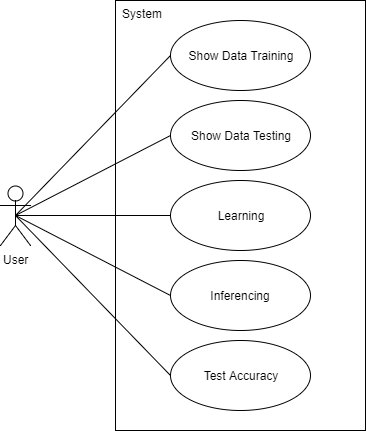
\includegraphics[width=6cm]{images/UseCase}
\end{figure}\\
\hline
\end{tabular}
\end{adjustbox}
\captionof{figure}{\itshape Use Case Diagram}
\end{table}

\subsection{{\itshape Class Diagram}}
\indent
Berikut merupakan {\itshape class} dan {\itshape method} yang akan digunakan dalam pembangunan sistem kategorisasi dokumen yang digambarkan dalam bentuk {\itshape class diagram}.

\begin{table}[H]
\begin{adjustbox}{width=1\textwidth}
\begin{tabular}{| p {14 cm} |}
\hline
\begin{figure}[H]
	\centering
	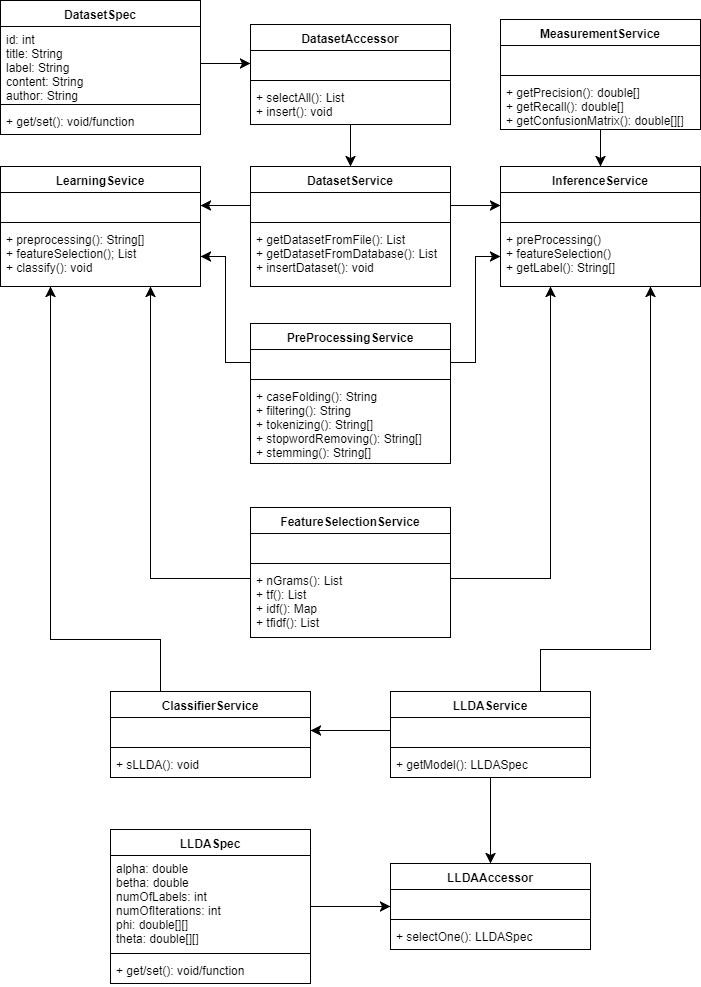
\includegraphics[width=7cm]{images/ClassDiagram}
\end{figure}\\
\hline
\end{tabular}
\end{adjustbox}
\captionof{figure}{\itshape Class Diagram}
\end{table}

\newpage